\documentclass[11pt]{article}
\renewcommand{\baselinestretch}{1.05}

\usepackage{amsmath,amsthm,verbatim,amssymb,amsfonts,amscd, graphicx}
\usepackage{graphics}

\usepackage{xcolor}

\usepackage[hidelinks]{hyperref}

\usepackage{parskip}

\renewcommand{\contentsname}{Table des mati\`eres}

\topmargin0.0cm
\headheight0.0cm
\headsep0.0cm
\oddsidemargin0.0cm
\textheight23.0cm
\textwidth16.5cm
\footskip1.0cm

\begin{document}

\title{\textbf{TP Caract\'erisation} }
\author{Lucien Dos Santos \\ Mohamed Hage Hassan}
\date{21 Mars, 2017}
\maketitle

\tableofcontents
\clearpage

\section{Introduction}

\section{Description G\'en\'erale}

Le but principal de ce TP est de caract\'eriser les 2 composantes principales du transistor MOS :

\begin{figure}[!htb]
\centering
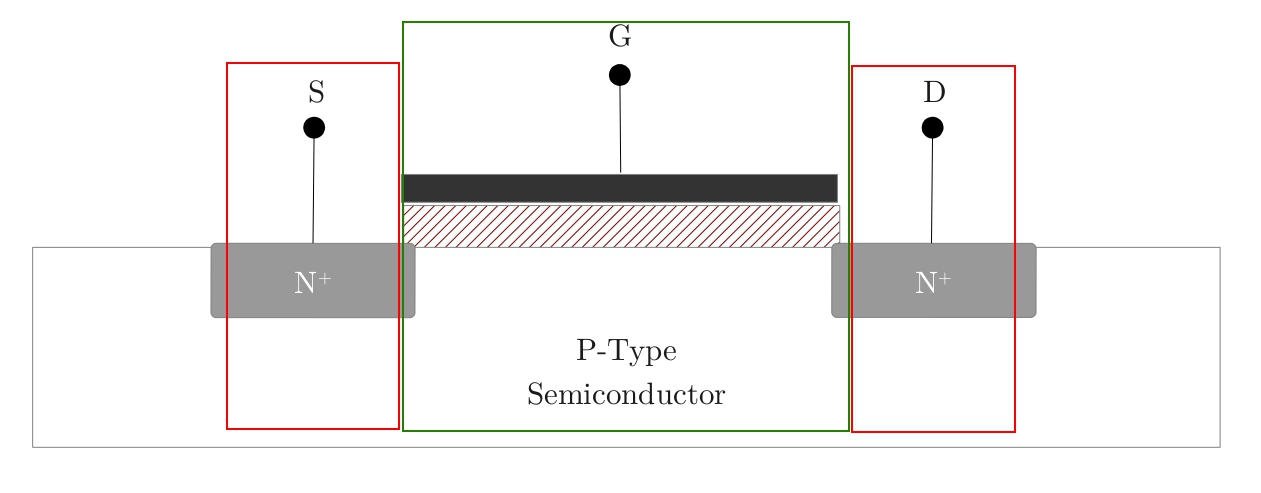
\includegraphics[scale=0.30]{mosfet_structure_implemented_side_view.jpg}
\caption{Composition du MOSFET}
\end{figure}

La capacit\'e MOS (vert) et les 2 jonctions PN (rouge) r\'esultantes des manipulations effectu\'ees en salle blanche.
On sp\'ecifie que ces 2 parties peut-\^etre utilis\'ees comme des composantes seules :

\begin{itemize}
\item \textbf{Jonction PN}

\begin{itemize}
\item[-] Capteurs thermiques (au lieu des couples thermiques).
\item[-] Capteurs optiques : photod\'eteteurs.
\item[-] Transmissions haute-fr\'equence (diode optiques).
\end{itemize}

\item \textbf{Capacit\'ees MOS}
\begin{itemize}
\item[-] Matrice de capacit\'ees MOS utilis\'ees pour la reconstruction d'une image dans les appareils photo r\'ecentes.
\end{itemize}

\end{itemize}

On note que pour la partie salle blanche, on a r\'ealiser la jonction PN :

\textbf{\'Etapes de r\'ealisation}
\begin{itemize}
\item[-] Nettoyage du wafer.
\item[-] D\'epot du $SiO_2$.
\item[-] Diffusion thermique pour le dopage du wafer (en type $n+$).
\item[-] Deposition d'une couche d'Aluminium
\item[-] Gravure d'aluminium.
\end{itemize}

\section{Caract\'erisation de la jonction PN}
On cherche \`a d\'eterminer la caract\'eristique I/V de la jonction.




\section{Conclusion}




\end{document}